% simple.tex - A simple article to illustrate document structure.

% preamble

\documentclass{article}
%% \usepackage{times}

\usepackage{float}
\usepackage{latexsym}
\usepackage{url}
\usepackage{graphicx}
\usepackage{natbib}
\usepackage{hyperref}
\hypersetup{colorlinks=true}
\usepackage{enumitem,amssymb}
\newlist{todolist}{itemize}{4}
\setlist[todolist]{label=$\square$}


\begin{document}

% top matter

\title{ALGORITHM DESIGN PROJECT}
\author{D\u{a}nciulescu Theodora - ioana }
\date{\today}
\maketitle

\begin{tabbing}
\indent{First Year}\\ 
\indent{Group: C.E.N 1.1A} \\
\indent{Web:}    \href{http://pt.becheru.net/project}{Programming Techniques}\\
\indent{Link to problem:}  \href{https://www.infoarena.ro/problema/order}{ORDER}\\
\end{tabbing}
\newpage
% sections
\section{Introduction}
The goal of my assignment is to develop a software for experimenting with algorithms. The project is focused on the development of skills for good programming of basic algorithms, covering coding, design, documentation and presentation of results. At the end of my project I must produce a set of deliverables including: a technical report, source code and experimental data.
I will present the usage of data structures and algorithms as RMQ Segment Trees and Binary Indexed Trees or Fenwick trees. 

\section{Problem statements} \label{sec:general}


There  are  N  children  (numbered  from  1  to  N)  placed  in  a  circle  formation  in  trigonometrical  sense.  We  will  see  that  this  trigonometrical  sense  doesn’t  even  matter.\\ 
At  each  step  i  (initially  1),  the  current  child  (initially  1)  starts  counting  i-children  in  this  trigonometrical  sense  and  the  child  it  reaches  is  excluded  from  the  circle.  The  child  after  the  eliminated  one  will  continue  the  count.  This  means  that  the  circle  will  eventually  be  empty.\\  
Our  task  is  to  print  the  order  in  which  the  children  are  excluded  from  the  circle.  

Example Explanation:
\begin{itemize}
    \item Input:  6  
    \item Output:  2  4  1  3  5  6  
    \item Explanation:  The  1st  child  starts  counting  (i  =  1),  so  we  reach  the  child  1+1=2  which  is  eliminated.  The  next  child  is  3.  children[]  =  {1,  3,  4,  5,  6}
    \item We  are  at  2nd  step,  so  we  count  2  children  starting  from  3  (inclusive).  We  reach  child  4.  Eliminated  child  4  will  pass  the  counting  responsibility  to  child  5.  children[]  =  {1,  3,  5,  6}
    \item Step  3,  count  3  children  from  5  (inclusive):  5,  6,  1.  We  eliminate  1,  next  child  is  3.  children[]  =  {3,  5,  6}
    \item Step  4,  count  4  children  from  3  (inclusive):  3,  5,  6,  3.  We  eliminate  3,  next  child  is  5.  children[]  =  {5,  6}
    \item Step  5,  count  5  children  from  5  (inclusive):  5,  6,  5,  6,  5.  We  eliminate  next  child  is  6.  children[]  =  {6}
    \item Step  6  and  last  step,  child  6  is  finally  removed.  
    \item So  the  erase  order  is:  2,  4,  1,  3,  5,  6.
\end{itemize}


\section{Algorithms} 
\subsection{SEGMENT TREES}
In computer science, a segment tree is a tree data structure for storing intervals, or segments. It allows querying which of the stored segments contain a given point. It can be implemented as a dynamic structure.\\

\subsubsection{How to build a segment tree}
\begin{itemize}
    \item There  might  be  more  ways  to  represent  a  Segment  Tree,  but  most  commonly  in  competitive  programming,  we’ll  see  this  method  of  representation:  
    \item A  1D  array  4  times  larger  in  dimension  than  the  number  of  elements.  Something  like  segtree[4*N].  
    \item Then  we  have:  
    \item  segtree[1]  -  the  information  of  the  root.  
    \item segtree[node]  –  information  in  our  current  node  \item segtree[node  *  2]  –  information  in  the  left  child  of  the  current  node  
    \item segtree[node  *  2  +  1]  –  information  in  the  right  child  of  the  current  node
    \item A  node  in  a  Segment  Tree  doesn’t  hold  information  about  a  single  element  of  the  input  array  (except  in  case  of  leaves),  but  rather  information  about  an  interval.  In  our  case/problem,  the  information  is  the  maximum  on  that  interval.  
    \item The  root  holds  information  about  the  whole  input  array,  so  interval  [1,  N].  We  split  this  interval  in  2  halves:  
    \begin{tabbing}
        \indent{} [1,  N/2]  –  this  left  half  is  the  responsibility  of  the  left  child  –  so  for    segtree[2*1]  =  segtree[2]  \\
        \\
        \indent{} [N/2+1,  N]  –  this  right  half  is  the  responsibility  of  the  right  child  –  so  for  segtree[2*1+1]  =  segtree[3]   \\   
    \end{tabbing}

    \item Applying  the  same  logic  recursively  will  then  build  our  whole  Segment  Tree!

\end{itemize}

\subsubsection{More info about Node Construction}
 We  know  the  maximum  of  a  single  element  already,  which  is  that  element.  That  means  we  know  the  information  for  the  leaves!  Any  interval  [x,  x]  has:
\begin{itemize}
    \item max([x,  x])  =  max(arr[x])  =  arr[x].
\end{itemize}

Suppose  we  are  in  the  node  with  interval  [x,  x+1].  Now  we  know  the  information  of  its  left  child  and  right  child.  So  we  use  both  information  to  compute  the  information  for  our  node.  In  our  case,  we  use  the  children  to  compute  the  maximum  for  our  node: 
\begin{itemize}
    \item max([x,  x+1])  =  max(max([x,x]), max([x+1,x+1]))=max(arr[x],  arr[x+1])
.
\end{itemize}
Now  we  can  safely  say  that  the  information  of  a  node  is  a  combination/computation  of  the  information  of  its  children. 
\\In  our  case:  segtree[node]  =  max(segtree[2*node],  segtree[2*node+1])
\\In  the  general  case:  segtree[node]  =  combine(segtree[2*node],  segtree[2*node+1]),  where  combine()  uses  that  information  however  it  needs  to  be  used.

\subsubsection{Update function}
When  we  want  to  modify  a  position  pos,  we  actually  want  to  modify  the  information  (maximum)  in  the  interval  [pos,  pos]  (leaf  node).  
\\We  will  reach  that  leaf  by  splitting  intervals  starting  from  the  root,  that  means  we  will  use  recurrence  to  get  to  the  leaf  node.  We  modify  the  information  in  the  leaf  node  and  also  update  the  parent  nodes  when  returning  to  them  from  the  recurrence.  
\\By  updating  the  parent  nodes  I  mean  reapplying  combine()  for  the  children.

\subsubsection{Query function}
Answering  a  Query  now  means  combining  information  from  the  biggest  intervals  possible  from  our  Segment  Tree  to  get  our  interval.  
\\Let’s  assume  we  have  the  Query  for  interval  [2,  5].
\\The  highest  intervals  we  can  get  from  our  tree  are:  [2,  2],  [3,  3],  [4,  5].  
\\Note  that,  even  though  [1,  2]  and  [1,  3]  are  bigger  than  [2,  2]  and  [3,  3],  using  their  information  would  mean  using  information  about  [1,  1]  too,  which  is  not  included  in  our  query  interval  [2,  5].  
\\How  do  we  get  the  biggest  intervals  possible?  We  start  from  the  root  and  start  splitting  intervals.  At  each  step  we  verify  if  the  interval  we  are  at  [left,  right]  is  included  in  the  query  interval  [a,  b]:  a  <=  left  and  right  <=  b.

\subsubsection{Time Complexity}
Segment Trees offers us a time complexity O(logN) for both Update and Query operation, and that is a very good complexity on any case.

\subsection{BINARY INDEXED TREES}

A Fenwick tree or binary indexed tree is a data structure that can efficiently update elements and calculate prefix sums in a table of numbers. This structure was proposed by Peter Fenwick in 1994 to improve the efficiency of arithmetic coding compression algorithms.
\\

\subsubsection{Time complexity and memory}

When compared with a flat array of numbers, the Fenwick tree achieves a much better balance between two operations: element update and prefix sum calculation. In a flat array of n numbers, you can either store the elements, or the prefix sums. In the first case, computing prefix sums requires linear time; in the second case, updating the array elements requires linear time (in both cases, the other operation can be performed in constant time). 
\\Fenwick trees allow both operations to be performed in  O(log n) time. This is achieved by representing the numbers as a tree, where the value of each node is the sum of the numbers in that subtree. The tree structure allows operations to be performed using only O(log n) node accesses.

\subsubsection{Constructing the intervals of a Binary Indexed Tree / Fenwick Tree}


\indent If all intervals have the same length for instance, the best balance is when we use $[$ $\sqrt{n}$ $]$ as the length of our intervals. This is a common technique when you know one of your operations takes B steps, and the other one N/B steps, we would pick B = $[$ $\sqrt{n}$ $]$, to minimize the worst case.

But we can get even better results if we consider the length of the interval ending at i to be the largest power of 2 that's a divisor of i.

Below you can see a graphical representation of the intervals, for N=16:

\begin{figure}[h!]
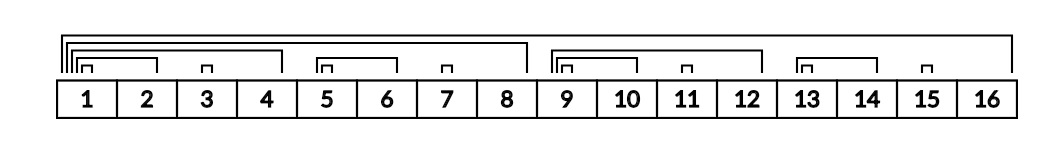
\includegraphics[scale=0.7]{aib_foto.jpg}
\end{figure}

These intervals may seem a bit chaotic at a first glance. 
\newline

\indent Let's say F$[$i$]$  is the length of the interval ending at index i. Basically are dealing with intervals of the form [i-F[i]+1, i]. For the example above F=[1,2,1,4,1,2,1,8,1,2,1,4,1,2,1,16]. 
\\
\indent We can show how to build F incrementally over lengths that are powers of 2:

\begin{itemize}
    \item if N = 1, it only makes sense to maintain an interval of length 1, so F=[1]
    \item The next step is for N=2. We will keep track of the first element and the sum of the first two, F=[1,2]:
    \item To find F for the next power of 2, we take the previous F, append a copy of it, and change the last element to be equal to N. So in the case of N=4, appending a copy to the previous F means we get [1, 2, 1, 2], but then we change the last element, so the new F=[1, 2, 1, 4]
    \item For N=8, we have F=[1,2,1,4,1,2,1,8]
    \item And for N=16, we get our result F=[1, 2, 1, 4, 1, 2, 1, 8, 1, 2, 1, 4, 1, 2, 1, 16]
\end{itemize}

\subsubsection{Finding all intervals that contain a certain index
}

\indent Since we've seen that intervals are either disjoint or fully contained one inside another, this part is equivalent with repeatedly just finding the next smallest interval that contains our own. Notice the father of an interval is always identified by a higher index, so we can say we need to find the difference between i and its father.

If i is a power of 2, the difference is equal to i, because the father is the next power of 2. Otherwise, we can again make use of the inductive way the Fenwick tree is build, and conclude that the difference for i is equal to the difference for i-p (p is the largest power of 2, smaller than i). 

You can already guess where this is going: the difference between an interval i and its father is equal to the interval's length which can be computed really fast with bitwise and operation between pos and -pos.

When we change to updating the interval ending at pos, its father's father, and so on.

In the function below we consider the first parameter to be the updated position, and the second one the difference between the new value and the old value being updated:

\begin{figure}[h!]
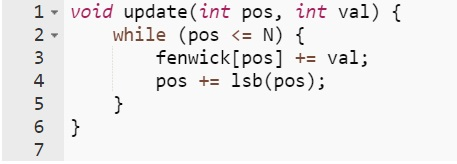
\includegraphics[scale=0.7]{query_aib_fotoexplanation.jpg}
\end{figure}

As for the query, we start at the index being queried, add the sum of its interval, and move to the left. This is where knowing the length of the intervals comes in handy:

\begin{figure}[h!]
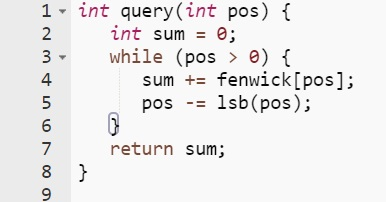
\includegraphics[scale=0.7]{query_aib_fotoexplanation_the_real.jpg}
\end{figure}


\section{Pseudocode Algorithms}

\subsection{General logic aspects of the problem}
Since  the  array  is  supposed  to  be  circular  (array[]  =  {2,  3,  4},  after  4  follows  2),    we  will  use  modulo.  Suppose  we  are  at  i-th  child  and  we  have  to  count  k  children  (inclusive).  Since  it’s  inclusive,  we  can  subtract  1  from  k.  Suppose  we  go  out  of  boundaries  i+k-1  >  remaining\_children.  We  can  use  modulo  to  get  out  dirt  and  provide  the  correct  position:  (i+k-1)  \%  remaining\_children.  That  was  easy.  But  what  if  the  result  is  0?  That  just  means  i+k-1  ==  remaining\_children,  so  we  set  our  result  to  remaining\_children.    
\\“But  wait,  if  we  start  counting  from  the  first  child,  he  is  not  included”.  That’s  fine,  we  will  just  start  using  the  formula  from  the  second  child,  not  from  the  first. 

\subsection{Segment Trees Method}
Suppose  we  know  the  position  of  the  child  we’d  like  to  remove  in  the  children[]  list  from  the  Example  Explanation.  We  know  that  at  each  step,  a  child  is  removed  from  that  list.  
\\What  if  we  build  a  ST  in  which  a  node’s  information  represents  how  many  children  from  that  node’s  interval  are  still  in  the  circle?  That’s  the  correct  idea,  by  the  way,  but  let’s  see  why  this  works.  

We  build  the  ST  before  any  counting,  that  means  the  circle  has  all  N  children.  
\\That  means  that  we  already  know  the  information  for  every  interval.  
\\How  many  children  are  in  an  interval  [a,  b]?  b-a+1,  of  course.  So  that  gets  rid  of  the  building  part  easily.  \\We  can  also  consider  knowing  information  only  about  a  leaf,  just  for  the  sake  of  it.  So  in  a  leaf  there  is  only  1  child.  Then  we  have  to  think  about  the  combine()  function  I  was  talking  about  in  the  Segment Trees General Aspect section.  
\\We  have  2  children  nodes  of  the  [a,  b]  interval  and  know  their  information:  
\begin{itemize}
    \item $[$a,  mid$]$ is interval A
    \item $[$mid+1,  b$]$ is interval B
\end{itemize}
where  mid=(a+b)/2  
\\Then  we  know  that  for  interval  [a,  b]  we  have  A+B  children  in  it.  
\\So  the  combine()  method  just  takes  both  values  of  the  children  and  sums  them  up.

Pseudocode for Building the Segment Tree

\begin{figure}[h!]
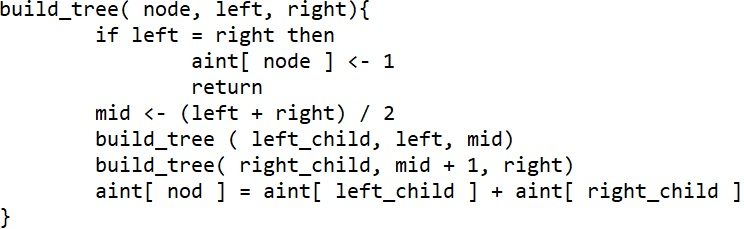
\includegraphics[scale=0.7]{pseudocod_build_st.jpg}
\end{figure}


When  do  we  need  to  UPDATE?  When  we  remove  a  child  from  the  circle.  
\\So  we  go  to  the  leaf  which  corresponds  to  that  child  and  subtract  1.  But  a  leaf  has  1  child  anyway,  so  we  can  just  set  it  to  0.  
\\Now  here  comes  the  tricky  part.  We  know  the  number  of  the  child  we  should  remove.  How  do  find  out  what  index  that  child  actually  has  (so  we  can  go  to  the  correct  leaf)?   
\\Let’s  take  a  concrete  example:  we  have  5  children  out  of  8  remaining.  
\\The  root  of  the  ST  has  interval  [1,  8].  Doing  updates  correctly,  we  should  have  segtree[root]=5.  
\\Suppose  the  left\_child  of  the  root  has  segtree$[$left\_child$]$ = 3. That  can  only  mean  segtree$[$right\_child$]$ = 5-3 = 2,  otherwise  the  tree  can’t  be  correct,  because  segtree$[$left\_child$]$+segtree$[$right\_child$]$ = segtree$[$parent$]$.


We  are  searching  the  leaf  of  the  2nd  child.  If  we  have  2  children  in  the  left\_child,  that  means  the  2nd  child  must  be  somewhere  in  that  interval,  so  we  go  to  the  left\_child.  But  what  if  we  looked  for  the  3rd  child?  There  are  only  2  children  in  the  left\_child,  so  the  3rd  must  be  somewhere  in  the  right\_child.  But if we go to the  right\_child,  are  we  still  looking  for  the  3rd  child  of  that  interval?  


We  know  that  in  the  left\_child  there  are  2  children,  so  that  means  2  children  are  already  excluded  from  our  search.  Left\_child  and  right\_child  are  basically  2  continuous  halves,  uniting  them  would  create  a  proper  big  interval.  Knowing  that  our  child  is  in  the  right\_child  means  we  know  that  in  this  big  interval  the  child  we’re  looking  for  is  somewhere  in  the  right  half.  That  means  already  half  of  the  big  interval  is  excluded  from  the  search.  So  in  the  right  half  we  are  not  looking  for  the  3rd  child  anymore,  but  rather  for  the  (3-2)=1st  child. 

We  reach  the  following  condition:  
\begin{itemize}
    \item if  (searched\_child $ <= $ segtree[left\_child])  go  search  for  searched\_child  in  left\_child
    \item else go  search  for  the  searched\_child $ -– $  segtree[left\_child]  in  the  right\_child
\end{itemize}    
In  other  words:  if  there  are  enough  children  in  the  left  half,  go  look  in  that  half,  otherwise,  go  look  in  the  remaining  interval  of  the  right  half.\\

Querying  here  actually  means  finding  the  index  of  the  child  we’re  looking  for.  And  that  is  basically  searching  in  the  same  way  as  when  updating,  but  instead  of  modifying  some  value,  we  just  return  the  index  of  that  leaf.  
\\As  you  can  see,  since  the  updateand  query  methods  do  the  same  thing  until  they  reach  the  leaf,  we  can  make  a  single  method  that  does  both  updateand  query  when  it  reaches  that  leaf.

Pseudocode for Query and Update function: 

\begin{figure}[h!]
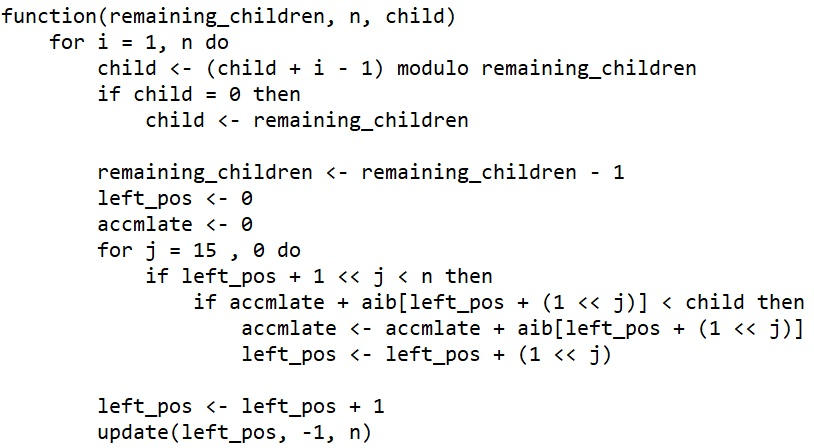
\includegraphics[scale=0.7]{function.jpg}
\end{figure}

Pseudocode for Order processing function:

\begin{figure}[h!]
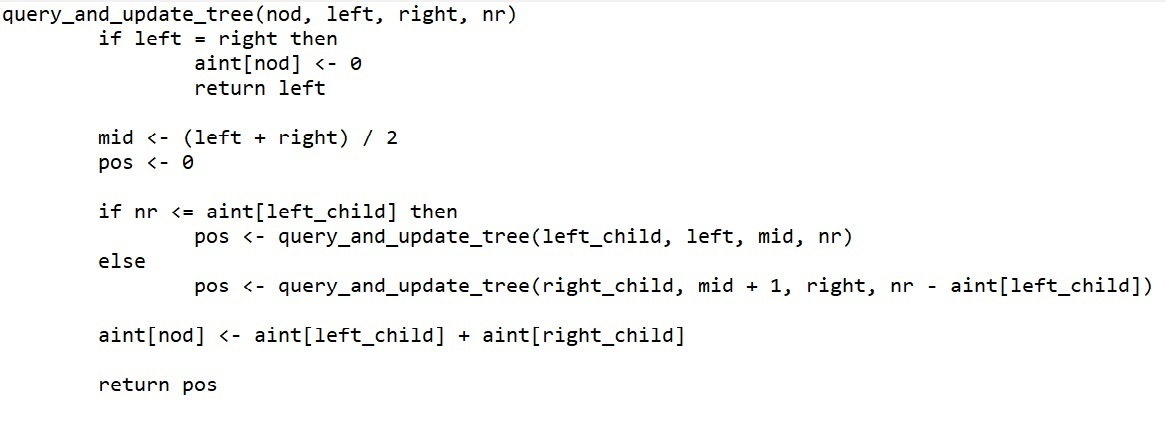
\includegraphics[scale=0.7]{query.jpg}
\end{figure}

\subsection{Binary Indexed Tree Method}

\indent In this method we will use the same formula described in the 4.1 General aspects of the problem section.
\newline
\indent We know that at every step a child is eliminated. We will initialize all the positions of the aib with 1 and when a child is eliminated we do update at that position with -1. So, the aib array for N = 6 will initially look like this :

\begin{figure}[h!]
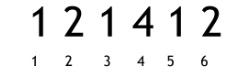
\includegraphics[scale=0.7]{n=6example_aib.jpg}
\end{figure}

\indent We will iterate through the aib array making use of as big as possible subsequences of length power of 2. For the above example we will have 2 on position 2, that means we have 2 children in the interval $[$1,2$]$, on position 4 we have the value 4, which means that in the interval $[$1,4$]$ we have 4 children. Depending on these values we will make a sort of binary search implemented on binary indexed trees like this: if we need to count more children we will look in the right of the current position, otherwise we will look in the left of the current position.

The aib array is a global variable so the modifications done to it in every function is applied globally.

\subsubsection{Update function}
\indent In this problem we notice that we only need the update function of binary indexed trees. The function has the classic parameters :  the position to update, the value to update with and the length of the aib array.

\begin{figure}[h!]
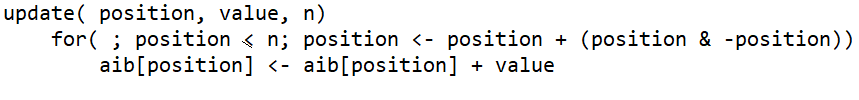
\includegraphics[scale=0.7]{update_for_aib.png}
\end{figure}

\subsubsection{Build AIB function}
We will initialize every position with 1, so we call the update function with the parameter position = 1 for every position from 1...n. 
The function has only one parameter, the lenght of the aib.

\begin{figure}[h!]
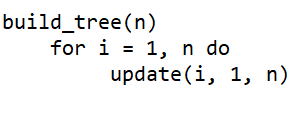
\includegraphics[scale=0.7]{build_aib.png}
\end{figure}

\subsubsection{Function generating the elimination of the children}

\indent At every step we must eliminate a child, using the formula I know which child to eliminate. We also decrease the variable remaining\_children. 
\indent For the binary search we set the bounds like this: left\_pos = 0, and the right bound I called it "accmlate" because it accumulates the number of children I counted and I set it as the right bound and equal to n. 

\indent As the problem states that the maximum number of children is 30.000, that means that it is also the maximum length of the aib array. That means that the maximum length is 2 at power 15. 

\indent I am iterating in decreasing order with a loop of length n through all the powers of 2 : 15....1;  at every position i check if the length power of 2 I am situated is lower than the length of my aib and I also check if  accmlate + the value at my iterated position is lower than the number of children to be counted. If the condition is full-filed I add the value from my iterated value to accmlate and actualize the left\_pos.

\indent Because I am starting with left\_pos from zero, before displaying the index of the eliminated child I increment it with 1, make update with -1 at that position and after that I display the position found.

\begin{figure}[h!]
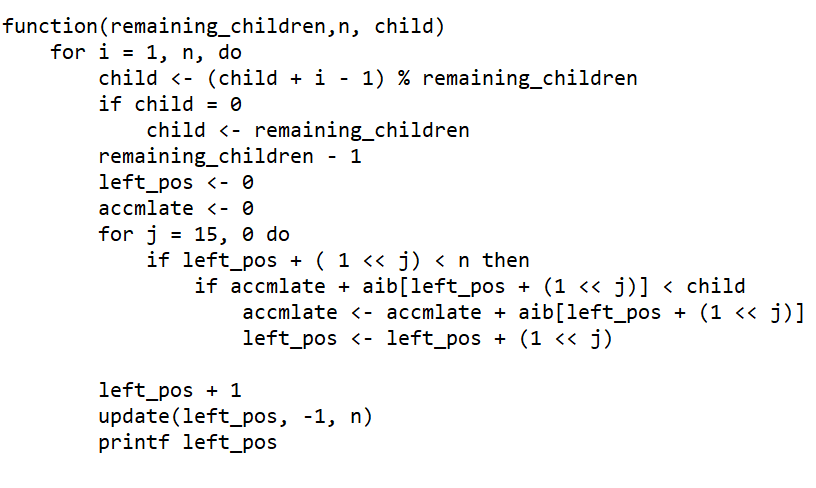
\includegraphics[scale=0.7]{function_aib_alg.png}
\end{figure}

\section{Application Design}

 The high level architectural overview of the application. 

\subsection{Segment Trees}

\begin{itemize}
    \item use of function to query and update the segment tree accordingly
    \item function to generate the order of elimination based on the data generated in my segment tree and also print it
    \item function to build the segment tree
    \item main function calling the other functions and initializing certain variables
\end{itemize}

\subsection{Binary Indexed Tree}
\begin{itemize}
    \item classic update function for binary indexed trees
    \item function to initialize the binary indexed tree
    \item function to compute the final answer using binary search on the data generated in the data structure used
    \item main function calling the other functions and initializing certain variables
\end{itemize}

\section{Experimental Data}

I use a c source to randomly generate my data. The input is represented by a single integer lower than 30000 which represents the number of children who plays the counting game. 

I simply genarate integers lower than 30000 and higher or equal than 1 with the standard function rand() from C library.

The time limit per test is 0.05 seconds and both methods pass all the tests successfully on the infoarena platform. 

\section{Results and Conclusions}

A segment tree is a tree data structure for storing intervals or segments. It allows querying which of the stored segments contain a given point. It is, in principle, a static structure; that is, its structure cannot be modified once it is built. A similar data structure is the interval tree.

A segment tree for a set I of n intervals uses O(n log n) storage and can be built in O(n log n) time. Segment trees support searching for all the intervals that contain a query point in O(log n + k), k being the number of retrieved intervals or segments.

Applications of the segment tree are in the areas of computational geometry, and geographic information system.

Fenwick tree or binary indexed tree is a data structure providing efficient methods for calculation and manipulation of the prefix sums of a table of values.Fenwick trees are used to implement the arithmetic coding algorithm. Development of operations it supports were primarily motivated by use in that case.

Using a Fenwick tree it is very easy to generate the cumulative sum table. From this cumulative sum table it is possible to calculate the summation of the frequencies in a certain range


% bibliography
\begin{thebibliography}{9}
\label{sec_ref}

	\bibitem{Wikipedia}
	\url{https://csacademy.com/lesson/fenwick_trees}
	  \emph{ Fenwick Trees }.
	  

	\bibitem{Traversal}
	\url{https://www.infoarena.ro/problema/arbint}
	  \emph{Segment Trees}.

\end{thebibliography}




\end{document}
